\section{Конструкторская часть}
В данном разделе будут представлена IDEF0 диаграмма метода, схемы алгоритма и структура приложения. Описан формат входных и выходных данных.

\subsection{IDEF0 диаграмма}
На рисунках \ref{idef0:top} -- \ref{idef0:A3} представленна IDEF0 диаграмма.

\begin{figure}[h]
	\begin{center}
		{\includegraphics[scale=0.5, angle=-90, page=1]{img/idef0.pdf}}
		\caption{IDEF0 диаграмма, верхний уровень}
		\label{idef0:top}
	\end{center}
\end{figure}

\begin{figure}[h]
	\begin{center}
		{\includegraphics[scale=0.5, angle=-90, page=2]{img/idef0.pdf}}
		\caption{IDEF0 диаграмма, декомпозиция А0}
		\label{idef0:A0}
	\end{center}
\end{figure}

\begin{figure}[h]
	\begin{center}
		{\includegraphics[scale=0.5, angle=-90, page=3]{img/idef0.pdf}}
		\caption{IDEF0 диаграмма, декомпозиция А1}
		\label{idef0:A1}
	\end{center}
\end{figure}

\begin{figure}[h]
	\begin{center}
		{\includegraphics[scale=0.5, angle=-90, page=4]{img/idef0.pdf}}
		\caption{IDEF0 диаграмма, декомпозиция А2}
		\label{idef0:A2}
	\end{center}
\end{figure}

\begin{figure}[h]
	\begin{center}
		{\includegraphics[scale=0.5, angle=-90, page=6]{img/idef0.pdf}}
		\caption{IDEF0 диаграмма, декомпозиция А3}
		\label{idef0:A3}
	\end{center}
\end{figure}

\subsection{Схемы алгоритмов}
На рисунках \ref{alg:main} - \ref{alg:schedule} представлены схемы ключевых алгоритмов программы.

\begin{figure}[h]
	\begin{center}
		{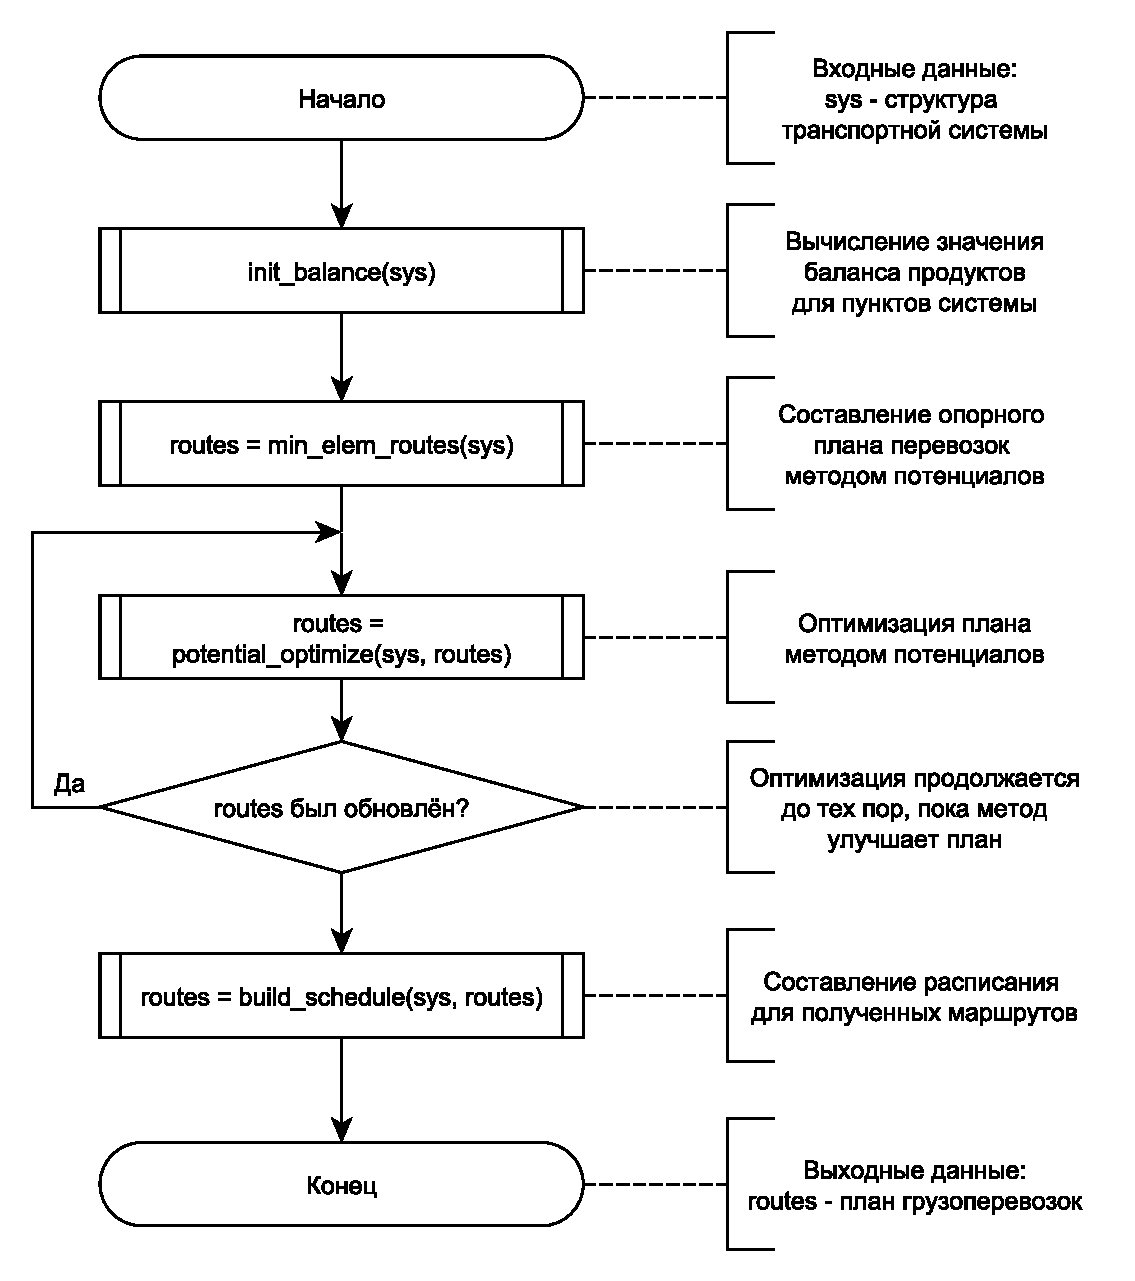
\includegraphics[scale=0.7, angle=0, page=1]{img/main_algorithm.pdf}}
		\caption{Схема общего алгоритма программы}
		\label{alg:main}
	\end{center}
\end{figure}

\begin{figure}[h]
	\begin{center}
		{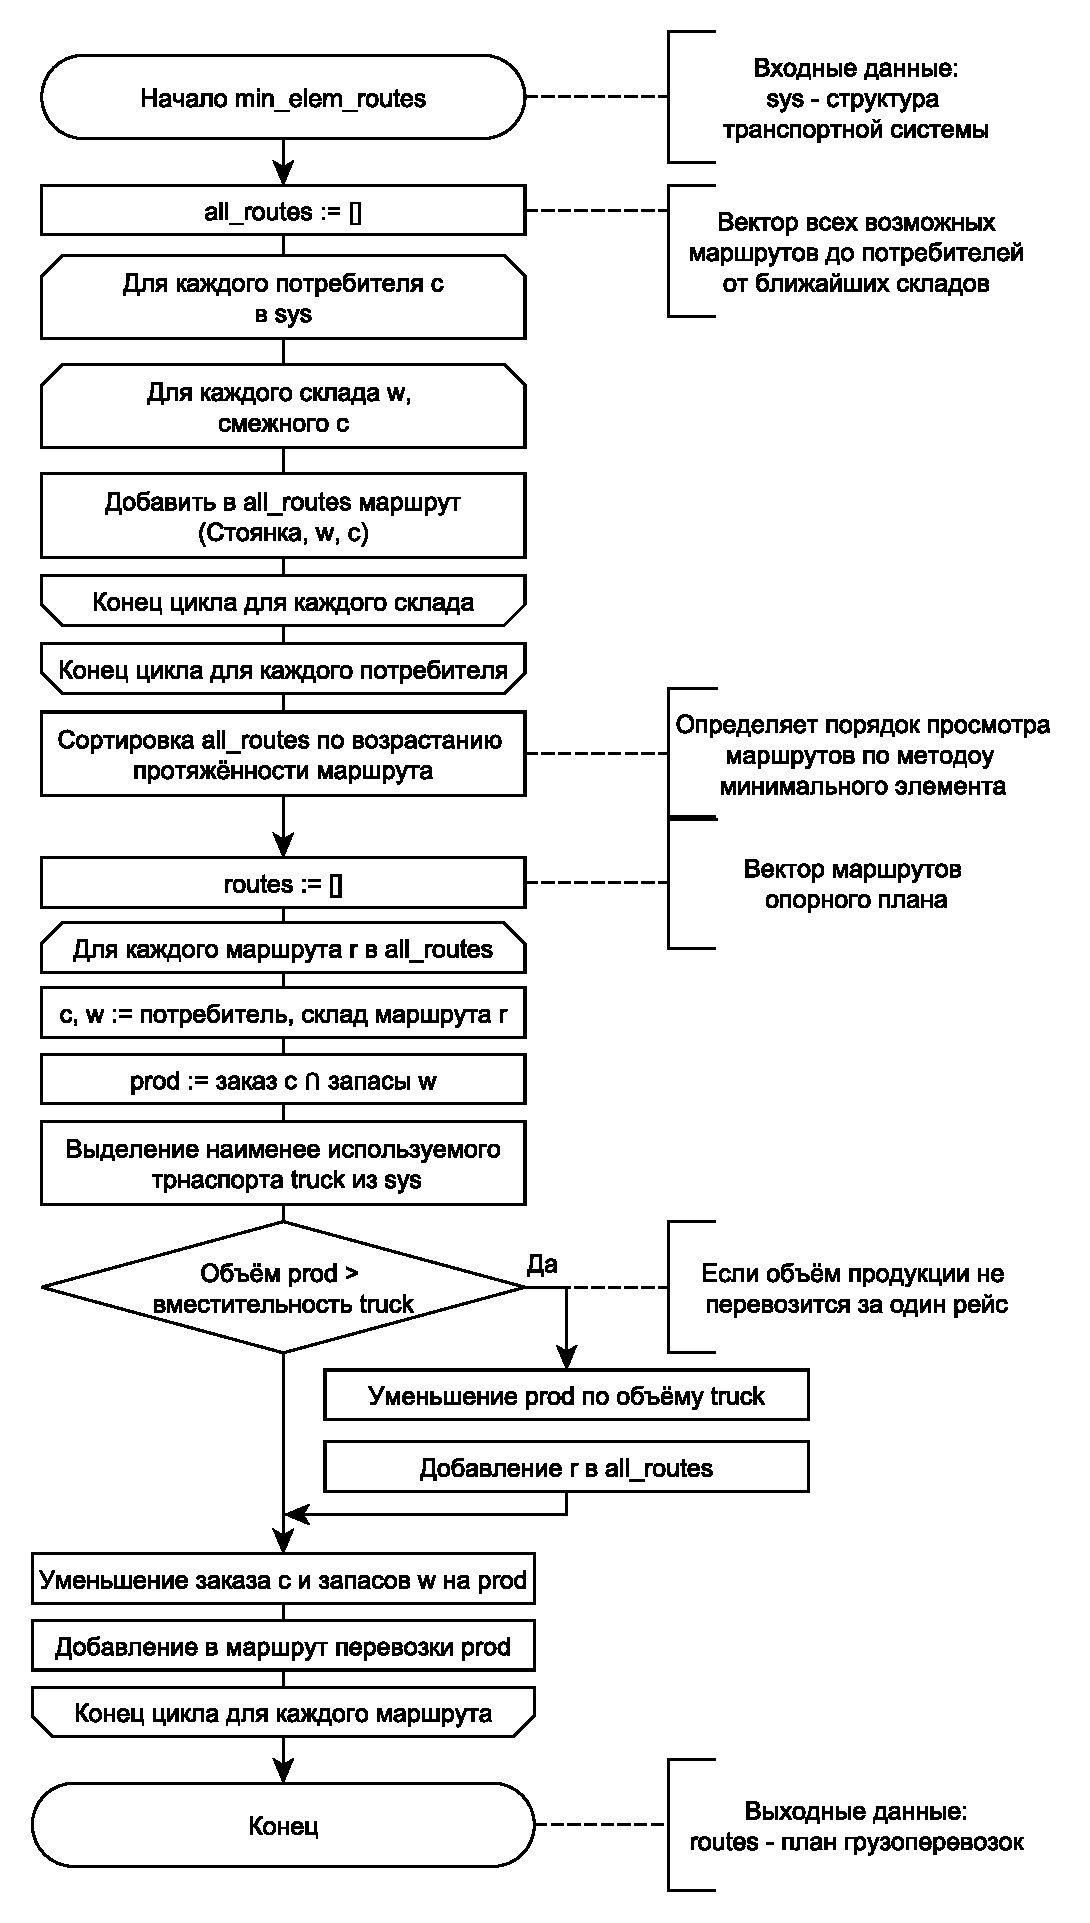
\includegraphics[scale=0.7, angle=0, page=1]{img/min_elem_routes.pdf}}
		\caption{Схема алгоритма минимального элемента}
		\label{alg:min_elem}
	\end{center}
\end{figure}

\begin{figure}[h]
	\begin{center}
		{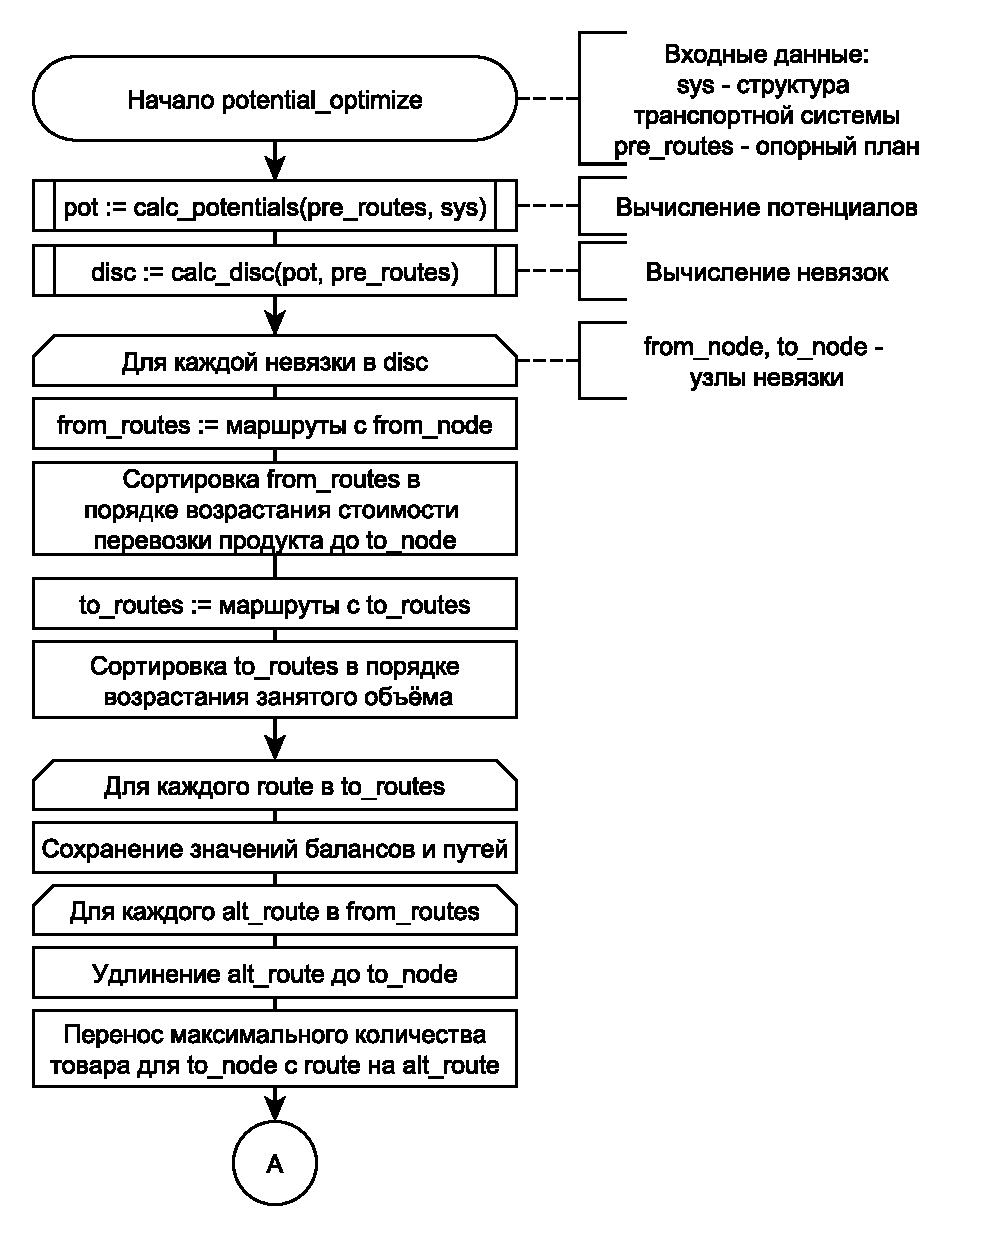
\includegraphics[scale=0.7, angle=0, page=1]{img/potential_optimize_1.pdf}}
		\caption{Схема алгоритма оптимизации методом потенциалов}
		\label{alg:potential_1}
	\end{center}
\end{figure}

\begin{figure}[h]
	\begin{center}
		{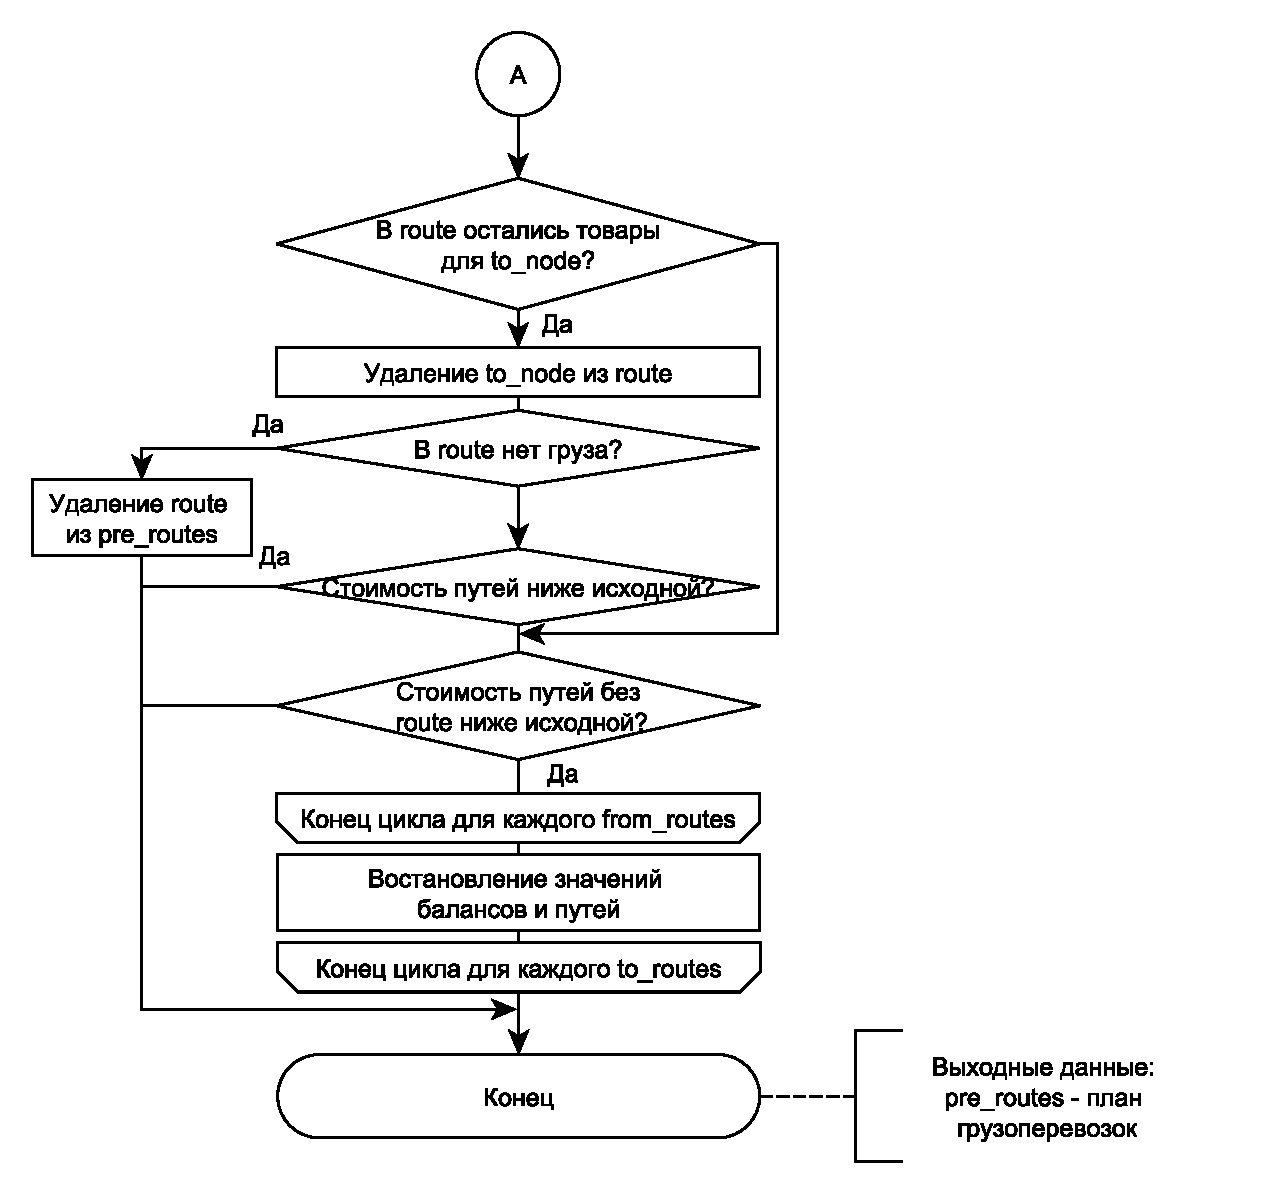
\includegraphics[scale=0.7, angle=0, page=1]{img/potential_optimize_2.pdf}}
		\caption{Схема алгоритма оптимизации методом потенциалов (продолжение)}
		\label{alg:potential_2}
	\end{center}
\end{figure}


\begin{figure}[h]
	\begin{center}
		{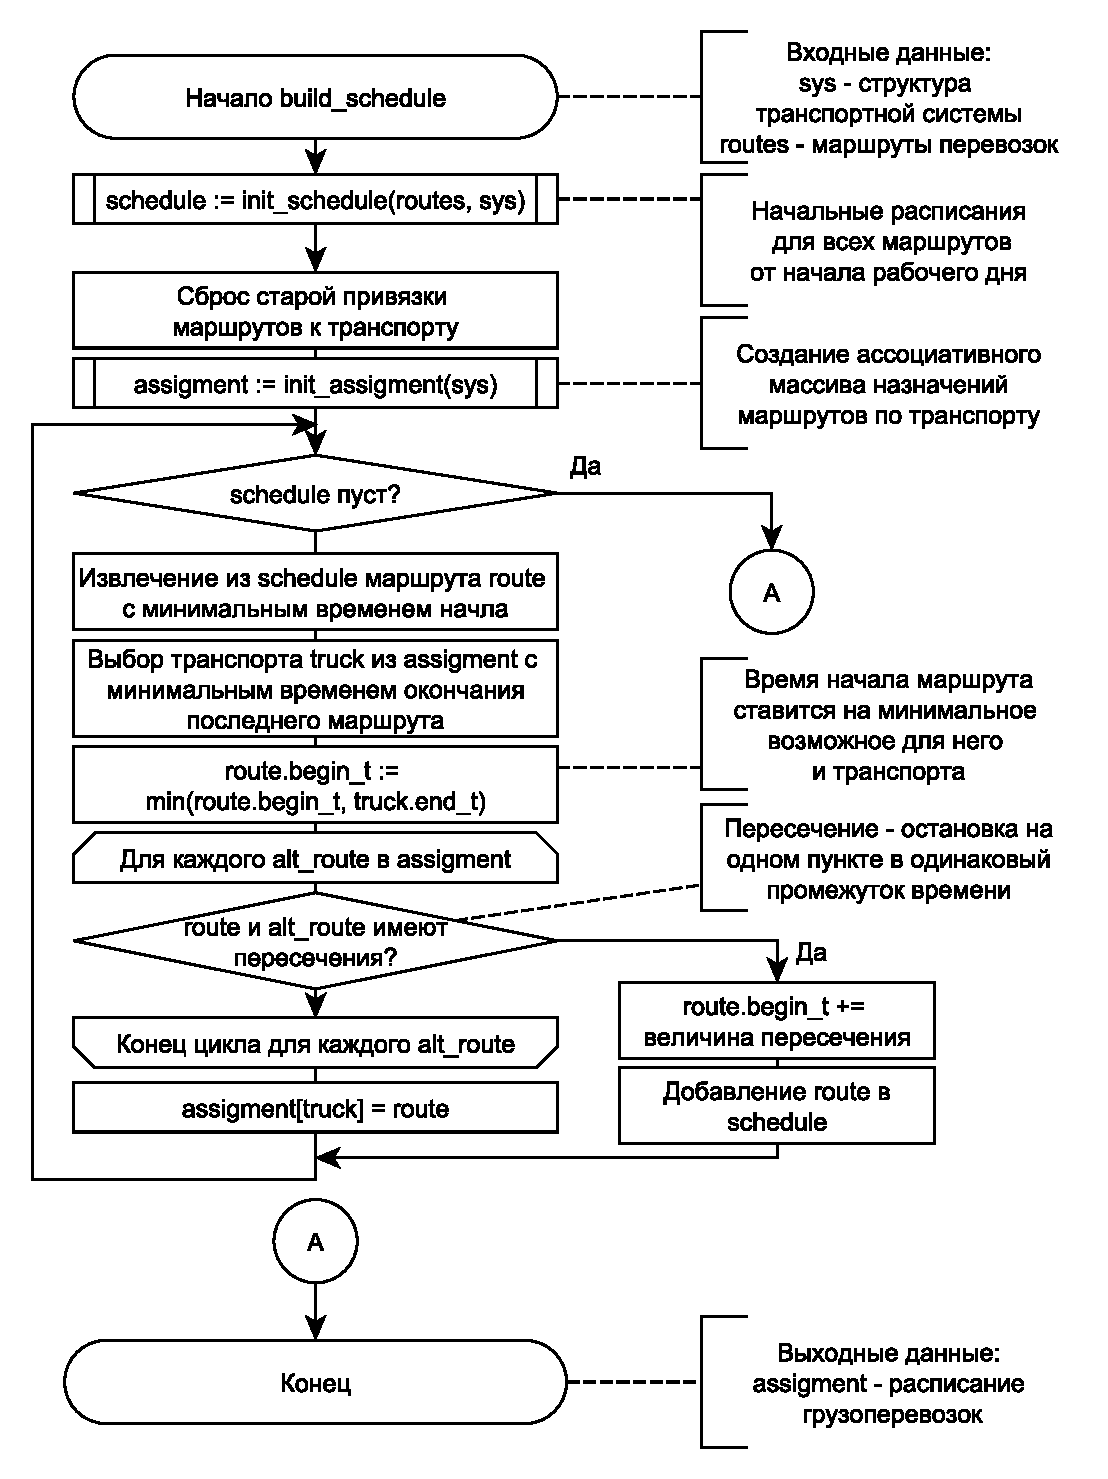
\includegraphics[scale=0.7, angle=0, page=1]{img/schedule.pdf}}
		\caption{Схема алгоритма составления расписания}
		\label{alg:schedule}
	\end{center}
\end{figure}

\pagebreak

\subsection{Схема сущностей транспортной системы}
В соответствии с ранее описанной математической моделью, в системе должны быть представлены сущности, изображённые на рисунке \ref{ER} ER-диаграммой.

\begin{figure}[h]
	\begin{center}
		{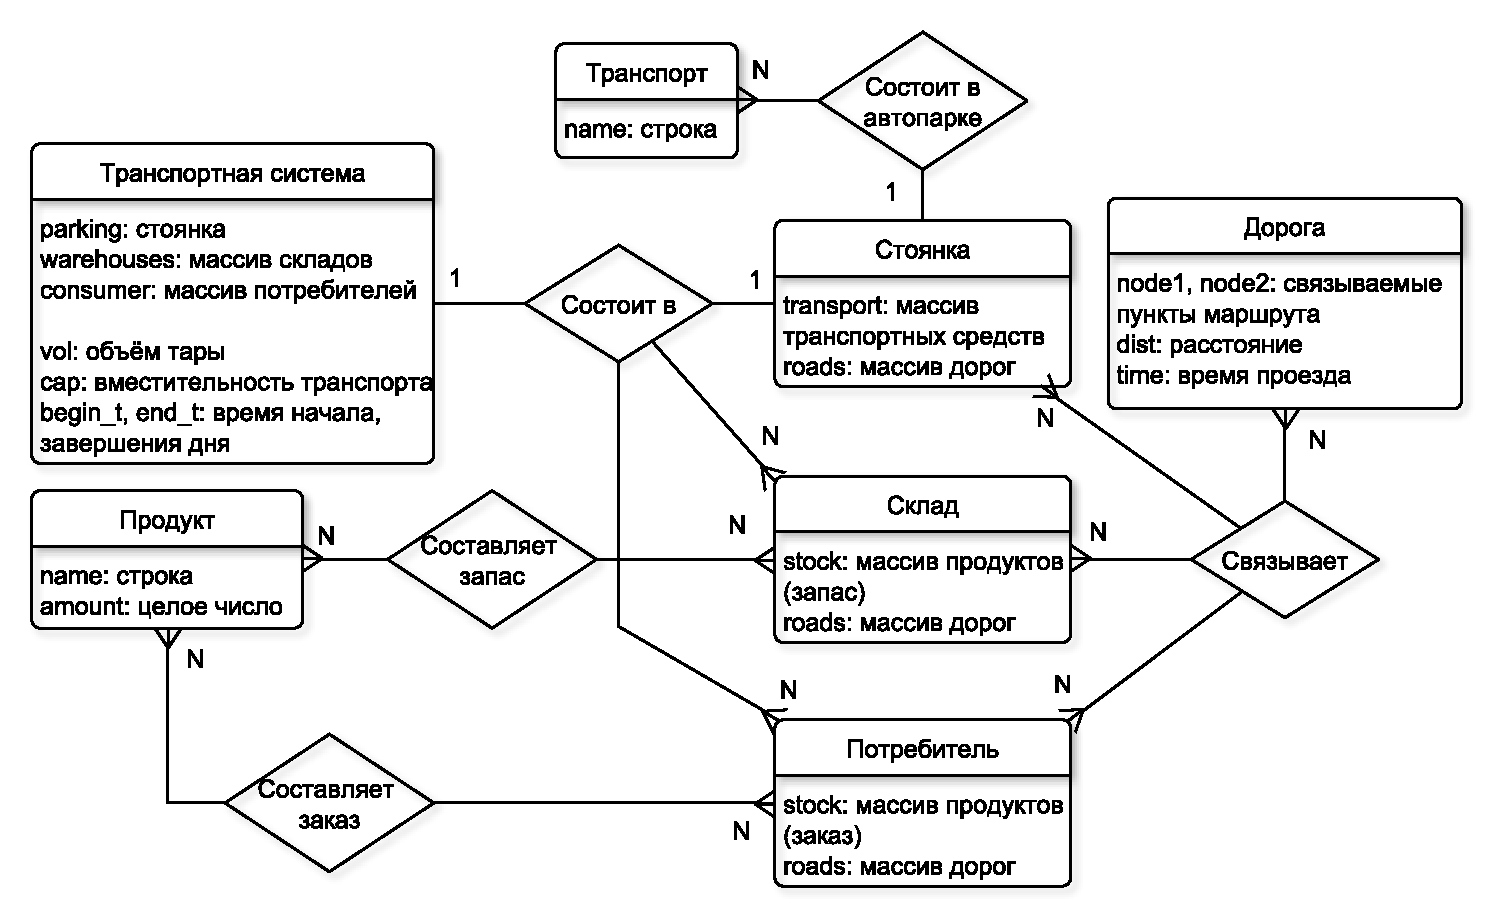
\includegraphics[scale=0.7, angle=0, page=1]{img/ER.pdf}}
		\caption{ER-диаграмма}
		\label{ER}
	\end{center}
\end{figure}

\pagebreak

\subsection{Формат входных данных}
В качестве входных данных выступает описание транспортной системы. Оно должно содержать в себе следующую информацию:

\begin{itemize}
	\item Список всех пунктов маршрута.
	\item Вместительность (в м$^3$) и количество транспорта.
	\item Список запасов складов. Каждый склад описывается списком продуктов (название и количество тар).
	\item Список заказов потребителей -- аналогично запасам складов.
	\item Список дорог: два связанных пункта, расстояние (в км.), время проезда (в мин.).
	\item Объём одной тары в (в м$^3$).
	\item Время начала и завершения рабочего дня.
\end{itemize}

\subsection{Формат выходных данных}
В качестве выходных данных выступает описание плана грузоперевозок. Оно состоит из списка маршрутов, каждый из которых должен содержать в себе следующую информацию:

\begin{itemize}
	\item Последовательность посещения пунктов.
	\item Номер привязанного транспортного средства.
	\item Список товаров, загружаемых или выгружаемых на каждом пункте.
	\item Список времени прибытия и отбытия в каждый пункт маршрута.
\end{itemize}	

\subsection*{Вывод}
В данном разделе были представленны IDEF0 и ER диаграммы, схемы алгоритмов. Описан формат входных и выходных данных программы.

\pagebreak